%android
\subsection{Description}\label{ssec:AndrDes}
\begin{floatingfigure}[r]{5cm}
	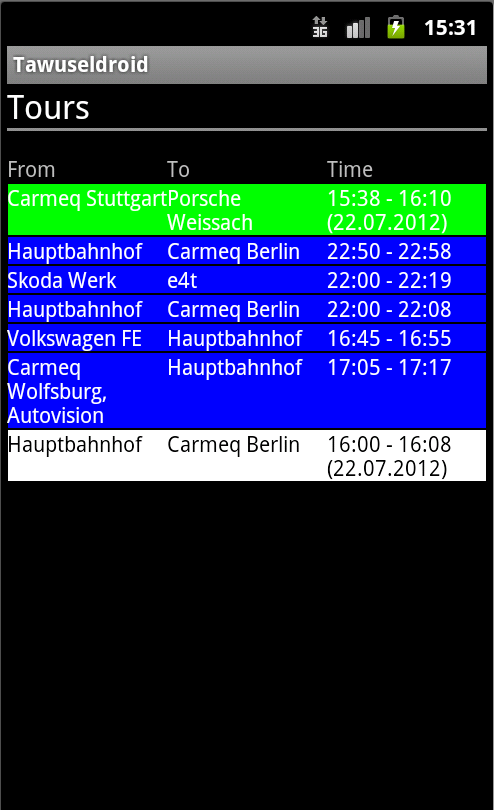
\includegraphics[width=4cm]{images/Tawuseldroid_tours.png}
	\caption{main view}
	\label{img:AndMV}
\end{floatingfigure}

\noindent
After the development of the key features of the TaWusel web service the team decided to implement an android app prototypically. This guarantees that all Carmeq employees who have access to an android phone can use the service more comfortable. The biggest advantage of an implementation of an android application is that the mobile phone doesn't need to have internet access at the whole time of the journey. On the other hand if one calls the web service with a web browser an internet connection is mandatory.

\emptyRow
The android application includes the most valuable features like creating a new tour or joining/leaving an existing tour. In figure \ref{img:AndMV} you can see the main view of the prototype. Like in the web service there is a table which is divided into three parts: the user's active tours, the templates to create a new to more comfortable and available tours created by other users. Since the application is a rough prototype the look and feel can be improved in most of the views, e.g. the colors of the tours table are just the standard android colors for green, blue and white to link their appearance to the corresponding entries in the web service.  

\emptyRow
\begin{floatingfigure}[l]{5cm}
	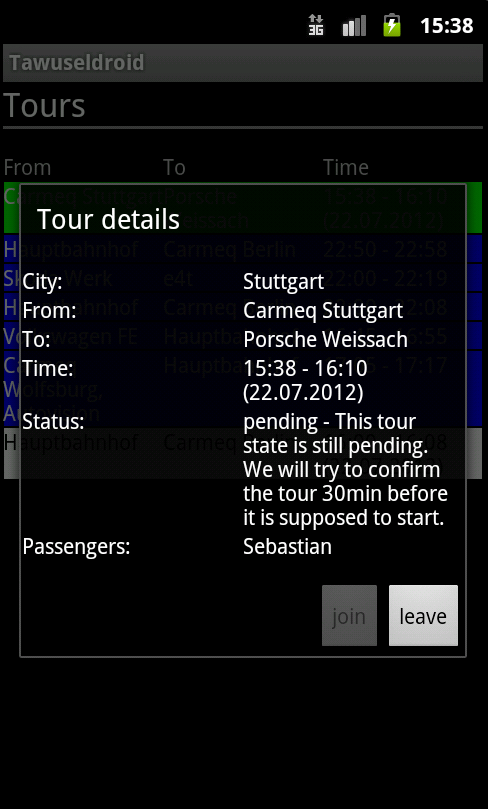
\includegraphics[width=4cm]{images/Tawuseldroid_details.png}
	\caption{details dialog}
	\label{img:AndDet}
\end{floatingfigure}
\noindent
By clicking on an existing tour a dialog is opened which shows more details according the chosen tour (see figure \ref{img:AndDet}). Here you find more information like the tour status or the passengers registered for it. For creating a new tour you can either pick a template (one of the blue rows) or click on the item "add tour" in the content menu. A dialog similar to the details dialog occurs. Here you can choose the city and the locations as well as the date and the time of the tour. To change the date as well as the departure or arrival time you just have to click on the corresponding field and a picker dialog appears.  A picture of the create dialog can be found in the appendix A in figure \ref{img:AndCD}.

\emptyRow
Unfortunately in the short period of development we were not able to implement a push function in the web service. So you have to fetch the tour data manually. For that reason just click on the item "update data" in the content menu. Remember that the mentioned activities call methods from the web service, therefore you need to have internet access.

\clearpage
\subsection{Architecture}\label{ssec:AndrArc}



\subsection{Installation guide}\label{ssec:AndrInst}

\begin{enumerate}
	\item Make sure you locate the tawusel.properties into the assets folder. Here you have to replace the json server property ("http://10.0.2.2:9000/") by the address of the server your tawusel service is running on.
	\item Generate your tawusel.apk. You can directly generate the apk from your eclipse project.
	\item Install the apk on your mobile phone.(Remark: the current version works stable on android 2.3.3 but its working on higher versions is not guaranteed)
\end{enumerate}
